\begin{frame}
	\frametitle{Proof of Work}
	\framesubtitle{metodo Hashcash}
	
	\begin{itemize}
	  \item nato per contrastare spam, DoS: serve un'operazione onerosa
	  \item \textit{facile} verificare che il messaggio è soluzione di problema \textit{difficile}
	  \item {\color{blue}brute force} unica tecnica risolutiva 
	  \item Problema: dati $h:\mathbb{Z}\rightarrow\mathbb{Z}_n,\,m,\,z \leq n$, trovare nonce $x:$
	  		%$$d=h(m|x) < T_z = \sum_{i=1}^{n-z}{2^i}$$ 
	  		$$d=\orange{h}(\orange{m}|\orange{x}) < T_z = \orange{2^{n-z+1}}$$
	   		\textit{i.e.} \textbf{digest ha $z$ zeri non significativi} (parametro {\color{blue}target})
	  		$$\Pr[d<T_z|Z=z]=\frac{1}{2^z} \Rightarrow \orange{O(2^z)}$$ %SAY dimensione media esponenziale della ricerca
	  \item problema risolto $\Leftrightarrow$ blocco $\mathfrak{B}$ risolto $\Leftrightarrow \{\mathfrak{T}\}_\mathfrak{B}$ convalidate  
	  \end{itemize}
\end{frame}
% ----------------------------------------------------------------------------------------------------------------------------
\begin{frame}
	\frametitle{Proof of Work}
	\framesubtitle{exempli gratia: $z=15$}	
	 
	$$ \mathrm{hash}(\mathrm{``hello\,world''}|001)=              9002381300129484192947128  $$
	$$ \vdots \;\;\;\;\;\;\;\;\;\;\;\;\;\;\;\;\;\;\;\;\;\;\;\;\;\;\;\;\;\; \vdots$$
	$$ \mathrm{hash}(\mathrm{``hello\,world''}|034)={\color{red}0000}834716283947104512438 $$
	$$ \vdots \;\;\;\;\;\;\;\;\;\;\;\;\;\;\;\;\;\;\;\;\;\;\;\;\;\;\;\;\;\; \vdots$$
	$$ \mathrm{hash}(\mathrm{``hello\,world''}|415)={\color{green}00000000000000000000}83201 $$
	\newline
	{\color{blue}n.b.} \textit{gambler's fallacy}
	$$\forall t_1,t_2 \;\;\; \Pr(Z=z, T=t_1)=\Pr(Z=z, T=t_2)$$

\end{frame}
% ----------------------------------------------------------------------------------------------------------------------------
\begin{frame}
	\frametitle{Proof of Work}
	\framesubtitle{adattamento target}
	
	\begin{itemize}
		\item target $z_i$ ricalcolato ogni 2016 blocchi risolti $\sim$ 2 settimane
		\item $\Delta_i \leftarrow t_{i} - t_{i-1}$
		\item $\Delta_i \leftarrow \mathrm{clip}(\Delta_i,\,0.5,\,8)$
		\item $z_{i+1} \leftarrow z_i\;\frac{\Delta_i}{2}$
		\item $z \propto \Delta \Rightarrow$ {\color{blue}soluzioni veloci} abbassano target 
			\newline $\;\;\;\;\text{\textit{i.e.}}$ generazione {\color{blue}problemi più difficili}, vv.
		\item blocco risolto mediamente ogni 10 minuti
	\end{itemize}
\end{frame}
% ----------------------------------------------------------------------------------------------------------------------------
\begin{frame}
	\frametitle{Proof of Work}
	\framesubtitle{sicurezza di SHA256}
	
	in teoria\ldots
	\begin{itemize}
		\item {\color{blue}preimage attack} attack: $O(2^{256})$
		\item {\color{blue}birthday attack}: $O(2^{\sfrac{256}{2}})$
	\end{itemize}
	
	\ldots in pratica
	
	\begin{table}
	    \begin{tabular}{l|l|l|l}
		    \textit{Metodo}             & \textit{Attacco}           & \textit{Iterazioni} & \textit{Complessità} \\ \hline
		    deterministico     & collisione        & 24         & $2^{28.5}$ \\  %TODO approfondire
		    meet in the middle & preimmagine       & 42         & $2^{248.4}$ \\ %TODO approfondire
		    differenziale      & pseudo collisione & 46         & $2^{178}$ \\
		    biclique           & preimmagine       & 45         & $2^{255.5}$ \\
	    \end{tabular}
	\end{table}
\end{frame}
% ----------------------------------------------------------------------------------------------------------------------------
\begin{frame}
	\frametitle{Proof of Work}
	\framesubtitle{prevenzione double spending}
	
	per spendere due volte la stessa $\mathfrak{T}$ occorre
	\begin{itemize}
		\item modificarne gli output $\Rightarrow \mathfrak{T}$ stessa $\Rightarrow \mathfrak{B}$ di appartenenza
		\item ricalcolare nonce $x$ per $\mathfrak{B}$ modificato
		\item modifica $\mathfrak{B} \Rightarrow $ modifica di $N$ blocchi successivi
		\item ricalcolare $N$ nonces $\Rightarrow$ risolvere $N$ problemi esponenziali
	\end{itemize}
	
	\vspace{1pt}
	
	\begin{figure}[H]
	 	\begin{center}
			 \begin{tabular}{c @{\hspace{1em}} c}
				 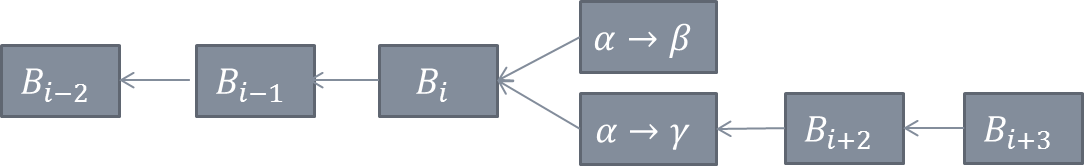
\includegraphics[width= 11cm]{images/dspending_ppt.png}
			 \end{tabular}
		 \end{center}
 	\end{figure}
 	{\color{blue}forking}
 	\begin{itemize}
 	  \item risolto imponendo aggiunta a ramo più lungo
 	  \item sotto ipotesi \textit{web of trust} sopravviverà il ramo corretto
 	\end{itemize}	
\end{frame}